% SOICT 2026 submission — Springer CCIS format (single-blind: keep author names).
% Requires the Springer LNCS/CCIS class `llncs.cls` + `splncs04.bst` from
% https://soict.org/wp-content/uploads/2025/09/Latex-Template-for-Springer.zip
% Max 12 pages excluding references. Figure: docs/paper/diagrams/soict_harlstmgat.{pdf,png}.
%
% VERSION 2026-09-07 FINAL: refreshed onto the latest canonical VolGA run (lookback 10, 7 walk-forward
%   folds, 5 seeds, horizon-matched volume->Parkinson edge). VN100 primary + VN30 cross-market;
%   HAR-X/LSTM/VolGA; all five metrics (MSE/RMSE/MAE/QLIKE/R2); DM split per market and contrast.
% All numbers read from
%   results/edge_hmatched/edgehm_{vn100,vn30}_h{1,5,10,22}.json
%   (metrics[model].{mse,rmse,mae,qlike,r2}, dm_date_clustered).
% Tables generated deterministically from those JSONs (see git history for the extractor).
\documentclass{llncs}
\usepackage{graphicx}
\graphicspath{{diagrams/}}   % figure lives in docs/paper/diagrams/ (do NOT add ./ — collides with output pdf)
\usepackage{booktabs}
\usepackage{amsmath}
\usepackage{placeins}
\usepackage[utf8]{inputenc}
\usepackage[T1,T5]{fontenc}

\begin{document}

\title{VolGA: A Graph-Attention Model for Stock Volatility Forecasting}

\author{Nguyễn Thành Quy\inst{1} \and Lê Trung Hoàng\inst{1} \and Trần Duy Hoàng\inst{1}}
\institute{University of Science, Vietnam National University Ho Chi Minh City, Ho Chi Minh City, Vietnam \\ \email{lthoang@hcmus.edu.vn}}

\maketitle

\begin{abstract}
Forecasting daily stock-price volatility --- how much a stock's price is likely to swing on a given
day --- is a core input to risk management and option pricing: a risk manager sizing exposure or a
trader pricing an option needs to know not only which direction a price may move but how large its swings will
be.

We propose \emph{VolGA} (Volatility Graph-Attention), a model that fuses a per-stock temporal branch
with a graph-attention branch, for multi-horizon volatility forecasting, using Vietnam's VN100 index
panel as the primary test market and the smaller VN30 panel as a cross-market study. All
feature-based models share the same five inputs and forecast a high--low range (Parkinson) measure of
daily variance, with the one-day-ahead ($h1$) horizon as the primary forecasting objective; the longer horizons $h5$ (one trading week), $h10$ (two trading weeks) and $h22$ (roughly one trading month) are reported as additional multi-horizon studies, against an extended HAR (HAR-X)
econometric benchmark and a same-feature no-graph LSTM that isolates the graph branch. Models are
compared with a leakage-free walk-forward protocol over multiple folds and five seeds on MSE, RMSE,
MAE, QLIKE and $R^2$, with a date-clustered Diebold--Mariano test that accounts for the
cross-sectional dependence of the panel. On VN100 at the daily horizon VolGA attains the lowest MSE,
RMSE, MAE and QLIKE and the highest $R^2$, and its QLIKE advantage over HAR-X is significant
($p=0.047$); relative to the no-graph LSTM the graph branch adds a significant QLIKE gain at the daily
horizon ($h1$: $p=0.006$), and against HAR-X VolGA's absolute-error advantage is significant at the
weekly horizon ($h5$: $p=0.001$). At the longer horizons the linear HAR-X is the strongest on QLIKE
and MSE, where the models are otherwise close. On the smaller VN30 panel VolGA leads on every metric
at the daily horizon, though its advantage over HAR-X is not statistically distinguishable; there the
graph branch's clearest effect is a significant absolute-error gain over the no-graph LSTM at the
daily, fortnightly and monthly horizons ($p<0.001$). The graph branch's QLIKE contribution is confined
to the broader, more actively traded VN100 panel at the daily horizon. Finally, training the deep
models directly on a QLIKE loss (rather than MSE) makes both the LSTM and VolGA significantly beat
HAR-X on QLIKE at the daily horizon on both panels ($p\le0.006$), at negligible cost to the
squared-error metrics.
\keywords{Volatility forecasting \and HAR \and LSTM \and Graph Attention Network \and Diebold--Mariano.}
\end{abstract}

\section{Introduction}
Financial markets are volatile: prices swing, and the size of those swings --- an asset's
\emph{volatility} --- is the standard measure of its risk. Because volatility drives how options
are priced, how much capital a position ties up, and how risk is budgeted across a portfolio,
forecasting it accurately is a long-standing problem in financial econometrics~\cite{corsi2009}.
Volatility is not observed directly; it is estimated from prices, so any forecast is a forecast of
an estimate. We target the daily \emph{Parkinson estimator}~\cite{parkinson1980}, which gauges a day's
variance from its high--low price range and uses more of the day's information than a close-to-close
measure; our
forecasting target is therefore a variance (a squared quantity), not a standard deviation.

The standard linear approach is the HAR family~\cite{corsi2009}: a plain linear regression that
predicts tomorrow's volatility from its own averages over the last day, the last week (about five
trading days), and the last month (about twenty-two), summarising volatility's long memory with a
handful of coefficients. This kind of model is deliberately simple yet provides a strong
low-complexity benchmark~\cite{corsi2009,audrino2025}; we adopt its extended form, HAR-X, which adds a
market factor and a volume regressor, as the linear benchmark throughout.

Two model families are widely proposed to capture information shared across stocks. Sequence models such as the
LSTM~\cite{lstm1997} learn non-linear patterns in a stock's own history, and graph neural networks
--- here a Graph Attention Network (GAT)~\cite{gat2018} --- capture \emph{cross-sectional dependence},
the same-day co-movement of turbulence across related stocks, by letting each stock draw on an
attention-weighted average of its most relevant peers; the graph is a predictive device, not an
identified economic spillover mechanism. Whether these additions improve
out-of-sample volatility forecasts is mixed in the literature, and reported gains are often
confounded by evaluation choices --- for example counting many co-moving stocks as independent
evidence, which overstates statistical significance.

This paper asks \emph{where}, if anywhere, deep and graph models improve on the linear HAR-X
benchmark. We take the VN100 index panel --- the larger, more actively traded of the
two panels we study --- as the primary test market and the smaller VN30 panel as a cross-market
study, and, holding the five inputs and the data design fixed, compare the extended HAR-X, a no-graph
LSTM, and VolGA under one leakage-free walk-forward protocol so the only difference is the model. The
headline finding is stated plainly: on the VN100 panel VolGA is strongest at the daily horizon,
attaining the lowest MSE, RMSE, MAE and QLIKE and the highest $R^2$, and its directed
volume$\to$Parkinson graph adds a significant QLIKE gain over the same-feature no-graph LSTM at the
daily horizon ($h1$: $p=0.006$); on the smaller VN30 panel VolGA again leads on every metric at the
daily horizon. Across both panels the linear HAR-X is the
strongest on QLIKE at the longer horizons, where the models are otherwise close, so the graph branch's
marginal value appears to track node breadth and trading activity.

Our contributions are: (i) a multi-horizon Vietnamese-market benchmark that holds the feature set
and data design fixed across HAR-X, a no-graph LSTM and VolGA on the VN100 and VN30 panels, so
any measured difference is attributable to a single component; (ii) the finding that VolGA delivers
the best daily-horizon accuracy across all five metrics on both panels and that the graph branch's
QLIKE contribution over the same-feature LSTM is significant on the larger, more actively traded VN100
panel at the daily horizon; and (iii) a Diebold--Mariano significance test clustered by trading date, which
avoids overstating significance for a cross-section of co-moving stocks~\cite{petersen2009}. Every reported number is taken from a stored results file.

\paragraph{Terminology.}
\emph{Volatility}: the size of a stock's price fluctuations, the standard proxy for its risk.
\emph{Parkinson estimator}: a day's variance measured from its high--low price range; our
forecasting target is this variance (squared units), not the standard deviation.
\emph{HAR}: a linear model predicting volatility from its own daily, weekly, and monthly averages.
\emph{HAR-X}: HAR augmented with exogenous regressors~\cite{corsi2009,clements2024}.
\emph{QLIKE}: a proxy-robust error measure for volatility forecasts that stays reliable when the
target is a noisy proxy; in the ratio-based implementation used here its asymmetric shape makes
forecast under- and over-shoots matter differently~\cite{patton2011}.
\emph{Diebold--Mariano (DM) test}: a test of whether one forecast is more accurate than another by
more than chance, computed from their day-by-day loss differences.
\emph{Graph Attention Network (GAT)}: a model in which stocks are nodes and edges carry influence;
each stock updates from an attention-weighted average of its neighbours, capturing cross-stock
\emph{spillover}.
\emph{Horizon} $h$: how many trading days ahead we forecast ($h\in\{1,5,10,22\}$, roughly a day,
week, fortnight, and month).

\section{Related Work}
\textbf{HAR and classical models.} HAR~\cite{corsi2009} approximates the long memory of realized
volatility with a daily/weekly/monthly cascade; recent work reports that rolling-window and
specification choices, rather than model class, often account for measured differences from
HAR~\cite{audrino2025}. The ``-X'' extension augments HAR with exogenous regressors; the low-frequency
OHLC HAR-X of Clements, Preve and Tee~\cite{clements2024} validates a range-based target, and
network-augmented HAR-X analogues have been proposed~\cite{gnarharx2025}.
\textbf{Deep and graph models.} LSTMs~\cite{lstm1997} are widely applied to financial series, and
graph neural networks model cross-asset spillovers, e.g.\ Graph Attention Networks~\cite{gat2018},
multivariate realized-volatility GNNs~\cite{chen2022} and spillover-aware GNN-HAR
hybrids~\cite{gnnhar2025}; reported effects vary across studies and data designs. Volatility spillover
measurement has a long econometric tradition~\cite{dy2012}. \textbf{Graph construction.} Our graph
uses a directed volume$\to$Parkinson relation (each node attends to its Top-5 volume-shock leaders,
edge-weighted, over two hops), motivated by the documented volume--volatility
association~\cite{karpoff1987} and used here as a predictive design choice rather than a causal claim.
\textbf{Evaluation.}
Volatility is latent, so we report the proxy-robust QLIKE metric~\cite{patton2011} alongside MSE, RMSE,
MAE and $R^2$; the learned models are trained with the MSE loss unless stated otherwise (the QLIKE-loss
ablation of Sec.~\ref{sec:qlikeloss} trains them directly on QLIKE), and QLIKE is otherwise an
evaluation-only metric.
Significance is assessed with the Diebold--Mariano test~\cite{dm1995} using the
Harvey--Leybourne--Newbold small-sample correction~\cite{hln1997}.

\section{Method}
\textbf{Target and features.} The target is the Parkinson variance~\cite{parkinson1980} at day
$t{+}h$, a non-negative point forecast. The primary target is the one-day-ahead horizon $h{=}1$;
the horizons $h\in\{5,10,22\}$ (one trading week, two weeks and roughly one trading month) are an
extended multi-horizon study reported for completeness. All three feature-based models (HAR-X, LSTM, VolGA) use the same five
node features per ticker at $t$: the daily Parkinson variance, its 5-day rolling mean (weekly), its
22-day rolling mean (monthly), a market Parkinson factor (the causal cross-sectional median of the
square-root Parkinson variance) and a 22-day volume z-score.

\textbf{Volatility estimator.} The target is the Parkinson variance. From the daily high $H$ and low
$L$ ($\ln$ is the natural logarithm), it estimates a day's variance from the high--low range:
\[
\sigma^2_{\mathrm{Park}} = \tfrac{1}{4\ln 2}\,\ln(H/L)^2 .
\]

\textbf{Models.} \emph{HAR-X} (linear benchmark~\cite{corsi2009,clements2024}): pooled OLS on the five
features (the daily/weekly/monthly cascade augmented with a market Parkinson factor and a volume
z-score), linear; its disclosed deviations from the canonical HAR-X are a range-based Parkinson target
and a direct single-day $t{+}h$ target. \emph{LSTM}: a two-layer LSTM (hidden 64) over the lookback
window of the five features; a single pooled model is trained over all tickers, each standardized by
its own scaler fit on training rows only, with a linear output inverse-transformed for evaluation. \emph{VolGA}
(Fig.~\ref{fig:arch}): the LSTM branch plus a Graph Attention Network branch~\cite{gat2018} that reads
the five node features at $t$ and attends over a directed volume$\to$Parkinson Top-5, edge-weighted,
two-hop graph estimated on training rows only; the branches are concatenated into an MLP head.
Comparing VolGA against the same-feature no-graph LSTM isolates the graph's contribution.

\textbf{Masked panel.} Not every stock is listed on every date. Rather than keep only the dates on
which all stocks trade (which discards most of the data), we keep every trading date and mask out
stocks not yet listed, with a mask-aware loss that ignores the masked stocks, so every model is
trained and evaluated on the same panel.

\textbf{Protocol.} We use an expanding-window walk-forward evaluation over multiple folds with a fixed
retrain cadence (the exact fold count and cadence are recorded in every results file so the runs are
reproducible; the runs reported here use seven folds), a lookback window of ten trading days, and five
seeds (batch size $32$; the seed set is fixed across models). For the learned models we report each
metric on the five-seed ensemble forecast, so the ranking reflects an average-across-seeds effect
rather than a single training run. We report MSE, RMSE, MAE, QLIKE and $R^2$; predictions are floored
at $10^{-2}$ times the per-node training mean, applied identically to every model. Significance uses
the \emph{date-clustered} Diebold--Mariano test on the five-seed ensemble (mean) forecast: the
per-observation loss differential is collapsed to one value per calendar date before the statistic
is computed. We report the targeted contrasts --- VolGA vs the
no-graph LSTM (the graph's marginal value) and VolGA vs HAR-X --- on three losses, because the
verdict can be loss-dependent: the QLIKE loss (as in the metrics tables), the squared-error loss
$(\hat{y}-y)^2$ whose mean is the MSE, and the absolute-error loss $|\hat{y}-y|$ whose mean is the MAE.
In the DM tables these three appear as the QLIKE, MSE and MAE columns. Per-metric
contrasts are reported without a multiple-comparison correction (unadjusted).

\begin{figure}[t]
\centering
% figure generated by docs/paper/diagrams/generate_arch.py -> diagrams/soict_harlstmgat.{pdf,png,svg}
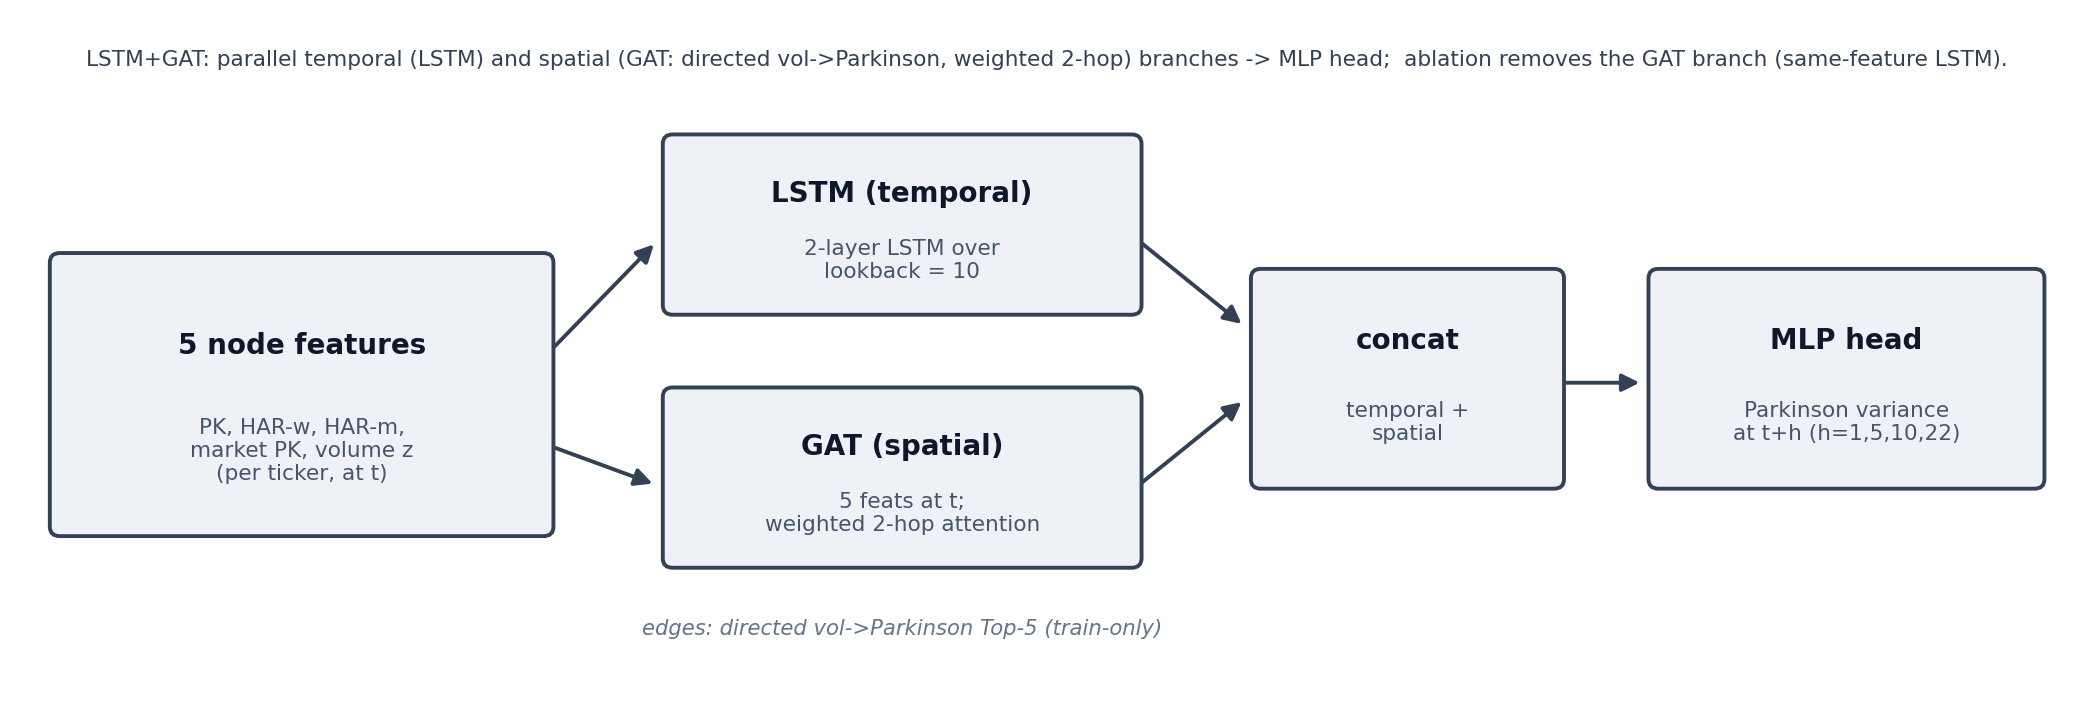
\includegraphics[width=\textwidth]{diagrams/soict_harlstmgat.png}
\caption{VolGA: a per-node LSTM temporal branch and a GAT spatial branch (directed volume$\to$Parkinson
Top-5 weighted two-hop attention) are concatenated into an MLP head; removing the GAT branch gives the
same-feature no-graph LSTM.}
\label{fig:arch}
\end{figure}

\section{Data}
The primary test market is the \textbf{VN100} index panel of the Vietnamese market (102 screened
tickers), the broader of the two panels; the \textbf{VN30} index panel (33 screened
tickers) serves as a cross-market study. Index membership follows the Ho Chi Minh Stock Exchange
index rules. Both use the masked panel of Sec.~3
with the five features, per-ticker standardization fit on training rows only, and the walk-forward
protocol above. The VN100 test sample is
46{,}512 masked observations at $h1$; the VN30 test sample is 12{,}936 masked observations at $h1$.

\section{Experiments}
The main comparison is the extended linear benchmark HAR-X and the proposed model VolGA (directed
volume$\to$Parkinson weighted two-hop) on the primary VN100 panel at horizons $\{1,5,10,22\}$,
reporting MSE, RMSE, MAE, QLIKE and $R^2$ and the date-clustered Diebold--Mariano test
(Table~\ref{tab:vn100main}). The ablation then adds the no-graph LSTM to isolate the graph branch on
VN100 (Sec.~\ref{sec:graph}) and repeats the comparison on the smaller VN30 panel (Sec.~\ref{sec:vn30}).

\begin{table}[t]
\centering
\caption{Main result --- primary market VN100 panel ($N=102$; 46{,}512 masked obs at $h1$; 7
walk-forward folds, 5 seeds; VolGA: five-seed ensemble point value). Lower is better on every metric
except $R^2$ (higher is better); best value in each row-pair in bold. MSE $\times10^{-7}$, RMSE/MAE
$\times10^{-4}$; QLIKE and $R^2$ unscaled.}
\label{tab:vn100main}
\footnotesize
\setlength{\tabcolsep}{6pt}
\begin{tabular}{llccccc}
\toprule
$h$ & Model & MSE & RMSE & MAE & QLIKE & $R^2$ \\
\midrule
1 & HAR-X & 2.356 & 4.853 & 2.845 & 0.5000 & 0.225 \\
1 & VolGA & \textbf{2.341} & \textbf{4.838} & \textbf{2.829} & \textbf{0.4879} & \textbf{0.230} \\
\midrule
5 & HAR-X & \textbf{2.590} & \textbf{5.089} & 3.105 & \textbf{0.5607} & \textbf{0.148} \\
5 & VolGA & 2.590 & 5.089 & \textbf{3.045} & 0.5662 & 0.148 \\
\midrule
10 & HAR-X & \textbf{2.739} & \textbf{5.233} & 3.242 & \textbf{0.5999} & \textbf{0.101} \\
10 & VolGA & 2.759 & 5.252 & \textbf{3.192} & 0.6127 & 0.094 \\
\midrule
22 & HAR-X & \textbf{2.874} & \textbf{5.361} & 3.423 & \textbf{0.6385} & \textbf{0.057} \\
22 & VolGA & 2.924 & 5.407 & \textbf{3.362} & 0.6476 & 0.041 \\
\bottomrule
\end{tabular}
\end{table}

\section{Results: the VN100 market}\label{sec:results}
On the primary VN100 panel (Table~\ref{tab:vn100main}) VolGA is strongest at the daily horizon: it
attains the lowest MSE, RMSE, MAE and QLIKE and the highest $R^2$ ($h1$ QLIKE $0.4879$ vs HAR-X
$0.5000$; $R^2$ $0.230$ vs $0.225$), and it has the lower MAE at every horizon. The date-clustered
contrast against HAR-X (Table~\ref{tab:dm-vn100-harx}) shows VolGA's QLIKE advantage is significant at
the daily horizon ($h1$: $p=0.047$) and its absolute-error advantage is significant at the weekly
horizon ($h5$: $p=0.001$). At the weekly, fortnightly and
monthly horizons the linear HAR-X is the strongest on QLIKE, MSE and $R^2$, where the two models are
otherwise close, and the QLIKE difference between them is not statistically distinguishable
($p=0.649$, $0.520$, $0.679$ at $h5$, $h10$, $h22$). VolGA therefore delivers the best daily-horizon
accuracy across every metric, with HAR-X competitive on QLIKE at the longer horizons.

\FloatBarrier
\section{Ablation studies}\label{sec:abl}
\subsection{Graph component (VN100)}\label{sec:graph}
Adding the no-graph LSTM to the primary comparison isolates the graph branch: removing the GAT branch
from VolGA gives the same-feature no-graph LSTM (Table~\ref{tab:vn100graph}), so the VolGA-vs-LSTM
contrast measures the graph's marginal value (Table~\ref{tab:dm-vn100-lstm}). On VN100 the graph adds
a significant QLIKE gain over the no-graph LSTM at the daily horizon ($h1$: $p=0.006$); at the weekly
horizon the QLIKE gain is in the same direction but not significant ($h5$: $p=0.083$). The trade-off
is visible on absolute error, where the no-graph LSTM is significantly lower at the daily horizon
($h1$: $p<0.001$) and at $h10$ ($p=0.010$): the graph improves the QLIKE-relevant calibration of the
daily forecast while the plain LSTM keeps the smaller mean absolute error. The significant VN100 graph
QLIKE gain is measured on the five-seed ensemble forecast and is best read as an average-across-seeds
effect rather than one guaranteed for a single training run.

\begin{table}[t]
\centering
\caption{Graph ablation --- VN100 panel: the no-graph LSTM vs the full VolGA (isolating the graph
branch; same scaling and sample as Table~\ref{tab:vn100main}; five-seed ensemble point value). Lower
is better on every metric except $R^2$ (higher is better); best value in each row-pair in bold. MSE
$\times10^{-7}$, RMSE/MAE $\times10^{-4}$; QLIKE and $R^2$ unscaled.}
\label{tab:vn100graph}
\footnotesize
\setlength{\tabcolsep}{6pt}
\begin{tabular}{llccccc}
\toprule
$h$ & Model & MSE & RMSE & MAE & QLIKE & $R^2$ \\
\midrule
1 & LSTM & 2.347 & 4.844 & \textbf{2.814} & 0.5155 & 0.228 \\
1 & VolGA & \textbf{2.341} & \textbf{4.838} & 2.829 & \textbf{0.4879} & \textbf{0.230} \\
\midrule
5 & LSTM & 2.594 & 5.093 & 3.046 & 0.5759 & 0.147 \\
5 & VolGA & \textbf{2.590} & \textbf{5.089} & \textbf{3.045} & \textbf{0.5662} & \textbf{0.148} \\
\midrule
10 & LSTM & \textbf{2.758} & \textbf{5.252} & \textbf{3.175} & \textbf{0.6127} & \textbf{0.094} \\
10 & VolGA & 2.759 & 5.252 & 3.192 & 0.6127 & 0.094 \\
\midrule
22 & LSTM & \textbf{2.918} & \textbf{5.402} & \textbf{3.351} & \textbf{0.6452} & \textbf{0.043} \\
22 & VolGA & 2.924 & 5.407 & 3.362 & 0.6476 & 0.041 \\
\bottomrule
\end{tabular}
\end{table}

\begin{table}[t]
\centering
\caption{Date-clustered DM contrasts on VN100 --- VolGA vs HAR-X ($p$-value; favoured model in
parentheses; bold when $p<0.05$; unadjusted).
The MSE and MAE columns give the DM test on the per-observation squared-error $(\hat{y}-y)^2$ and absolute-error $|\hat{y}-y|$ losses (whose means are the MSE and MAE).}
\label{tab:dm-vn100-harx}
\footnotesize
\setlength{\tabcolsep}{8pt}
\begin{tabular}{lccc}
\toprule
$h$ & QLIKE & MSE & MAE \\
\midrule
1 & \textbf{0.047 (VolGA)} & 0.273 (VolGA) & 0.083 (VolGA) \\
5 & 0.649 (HAR-X) & 0.973 (HAR-X) & \textbf{0.001 (VolGA)} \\
10 & 0.520 (HAR-X) & 0.321 (HAR-X) & 0.086 (VolGA) \\
22 & 0.679 (HAR-X) & 0.100 (HAR-X) & 0.224 (VolGA) \\
\bottomrule
\end{tabular}
\end{table}

\begin{table}[t]
\centering
\caption{Date-clustered DM contrasts on VN100 --- VolGA vs the same-feature no-graph LSTM (the graph's
marginal value; $p$-value; favoured model in parentheses; bold when $p<0.05$; unadjusted). The MSE and MAE columns give the DM test on the per-observation squared-error $(\hat{y}-y)^2$ and absolute-error $|\hat{y}-y|$ losses (whose means are the MSE and MAE).}
\label{tab:dm-vn100-lstm}
\footnotesize
\setlength{\tabcolsep}{8pt}
\begin{tabular}{lccc}
\toprule
$h$ & QLIKE & MSE & MAE \\
\midrule
1 & \textbf{0.006 (VolGA)} & 0.274 (VolGA) & \textbf{$<$0.001 (LSTM)} \\
5 & 0.083 (VolGA) & 0.288 (VolGA) & 0.779 (VolGA) \\
10 & 0.989 (LSTM) & 0.872 (LSTM) & \textbf{0.010 (LSTM)} \\
22 & 0.329 (LSTM) & 0.176 (LSTM) & 0.223 (LSTM) \\
\bottomrule
\end{tabular}
\end{table}

\subsection{Other market: VN30}\label{sec:vn30}
Repeating the comparison on the smaller VN30 panel (Table~\ref{tab:vn30main}; the graph ablation is in
Table~\ref{tab:vn30graph}) VolGA again leads at the
daily horizon: it has the lowest MSE, RMSE, MAE and QLIKE and the highest $R^2$ at $h1$. Against HAR-X,
however, none of the VolGA differences are statistically distinguishable at any horizon
(Table~\ref{tab:dm-vn30-harx}; $h1$ QLIKE $p=0.280$, absolute error $p=0.162$), so on this smaller
panel VolGA's daily-horizon lead is not significant. The graph's marginal value over the no-graph LSTM
(Table~\ref{tab:dm-vn30-lstm}) is a significant absolute-error gain at the daily, fortnightly and
monthly horizons ($p<0.001$), while the QLIKE contrast is not statistically distinguishable at any
horizon. The graph branch thus contributes a significant QLIKE gain only on the broader, more actively
traded VN100 panel, at the daily horizon.

\begin{table}[t]
\centering
\caption{Cross-market main result --- VN30 panel ($N=33$; 12{,}936 masked obs at $h1$; 7 folds, 5
seeds; VolGA: five-seed ensemble point value). Lower is better on every metric except $R^2$ (higher is
better); best value in each row-pair in bold. MSE $\times10^{-7}$, RMSE/MAE $\times10^{-4}$; QLIKE and
$R^2$ unscaled.}
\label{tab:vn30main}
\footnotesize
\setlength{\tabcolsep}{6pt}
\begin{tabular}{llccccc}
\toprule
$h$ & Model & MSE & RMSE & MAE & QLIKE & $R^2$ \\
\midrule
1 & HAR-X & 2.093 & 4.575 & 2.547 & 0.4801 & 0.260 \\
1 & VolGA & \textbf{2.080} & \textbf{4.561} & \textbf{2.530} & \textbf{0.4740} & \textbf{0.264} \\
\midrule
5 & HAR-X & \textbf{2.182} & \textbf{4.671} & \textbf{2.682} & \textbf{0.5602} & \textbf{0.175} \\
5 & VolGA & 2.195 & 4.685 & 2.693 & 0.5672 & 0.170 \\
\midrule
10 & HAR-X & \textbf{2.352} & \textbf{4.850} & 2.862 & 0.6091 & \textbf{0.120} \\
10 & VolGA & 2.359 & 4.857 & \textbf{2.827} & \textbf{0.6061} & 0.118 \\
\midrule
22 & HAR-X & \textbf{2.844} & \textbf{5.333} & \textbf{3.090} & \textbf{0.6782} & \textbf{0.076} \\
22 & VolGA & 2.895 & 5.381 & 3.094 & 0.6882 & 0.060 \\
\bottomrule
\end{tabular}
\end{table}

\begin{table}[t]
\centering
\caption{Cross-market graph ablation --- VN30 panel: the no-graph LSTM vs the full VolGA (isolating the graph branch; same sample as Table~\ref{tab:vn30main}; five-seed ensemble point value). Lower is better on every metric except $R^2$ (higher is better); best value in each row-pair in bold. MSE $\times10^{-7}$, RMSE/MAE $\times10^{-4}$; QLIKE and $R^2$ unscaled.}
\label{tab:vn30graph}
\footnotesize
\setlength{\tabcolsep}{6pt}
\begin{tabular}{llccccc}
\toprule
$h$ & Model & MSE & RMSE & MAE & QLIKE & $R^2$ \\
\midrule
1 & LSTM & \textbf{2.079} & \textbf{4.560} & 2.560 & 0.4787 & \textbf{0.265} \\
1 & VolGA & 2.080 & 4.561 & \textbf{2.530} & \textbf{0.4740} & 0.264 \\
\midrule
5 & LSTM & 2.197 & 4.687 & 2.703 & 0.5738 & 0.169 \\
5 & VolGA & \textbf{2.195} & \textbf{4.685} & \textbf{2.693} & \textbf{0.5672} & \textbf{0.170} \\
\midrule
10 & LSTM & 2.361 & 4.859 & 2.848 & \textbf{0.6048} & 0.117 \\
10 & VolGA & \textbf{2.359} & \textbf{4.857} & \textbf{2.827} & 0.6061 & \textbf{0.118} \\
\midrule
22 & LSTM & 2.898 & 5.383 & 3.132 & \textbf{0.6832} & 0.059 \\
22 & VolGA & \textbf{2.895} & \textbf{5.381} & \textbf{3.094} & 0.6882 & \textbf{0.060} \\
\bottomrule
\end{tabular}
\end{table}

\begin{table}[t]
\centering
\caption{Date-clustered DM contrasts on VN30 --- VolGA vs HAR-X ($p$-value; favoured model in
parentheses; bold when $p<0.05$; unadjusted).
The MSE and MAE columns give the DM test on the per-observation squared-error $(\hat{y}-y)^2$ and absolute-error $|\hat{y}-y|$ losses (whose means are the MSE and MAE).}
\label{tab:dm-vn30-harx}
\footnotesize
\setlength{\tabcolsep}{8pt}
\begin{tabular}{lccc}
\toprule
$h$ & QLIKE & MSE & MAE \\
\midrule
1 & 0.280 (VolGA) & 0.576 (VolGA) & 0.162 (VolGA) \\
5 & 0.652 (HAR-X) & 0.510 (HAR-X) & 0.643 (HAR-X) \\
10 & 0.843 (VolGA) & 0.717 (HAR-X) & 0.114 (VolGA) \\
22 & 0.756 (HAR-X) & 0.207 (HAR-X) & 0.929 (HAR-X) \\
\bottomrule
\end{tabular}
\end{table}

\begin{table}[t]
\centering
\caption{Date-clustered DM contrasts on VN30 --- VolGA vs the same-feature no-graph LSTM (the graph's
marginal value; $p$-value; favoured model in parentheses; bold when $p<0.05$; unadjusted). The MSE and MAE columns give the DM test on the per-observation squared-error $(\hat{y}-y)^2$ and absolute-error $|\hat{y}-y|$ losses (whose means are the MSE and MAE).}
\label{tab:dm-vn30-lstm}
\footnotesize
\setlength{\tabcolsep}{8pt}
\begin{tabular}{lccc}
\toprule
$h$ & QLIKE & MSE & MAE \\
\midrule
1 & 0.201 (VolGA) & 0.909 (LSTM) & \textbf{$<$0.001 (VolGA)} \\
5 & 0.156 (VolGA) & 0.704 (VolGA) & 0.080 (VolGA) \\
10 & 0.691 (LSTM) & 0.801 (VolGA) & \textbf{$<$0.001 (VolGA)} \\
22 & 0.595 (LSTM) & 0.779 (VolGA) & \textbf{$<$0.001 (VolGA)} \\
\bottomrule
\end{tabular}
\end{table}

\subsection{Training objective: QLIKE-loss training}\label{sec:qlikeloss}
The main results train the deep models on the MSE loss (Sec.~3), on which HAR-X is the strongest on
QLIKE at the weekly and longer horizons. Because QLIKE is the evaluation target, we also train the
LSTM and VolGA directly on a QLIKE loss and re-evaluate (Table~\ref{tab:qlikeloss}). QLIKE-loss
training lowers the deep models' QLIKE at almost every horizon and, at the daily horizon, makes both
significantly beat HAR-X on QLIKE on both panels (date-clustered DM --- VN100: LSTM $p=0.003$, VolGA
$p=0.004$; VN30: LSTM $p=0.004$, VolGA $p=0.006$). This removes the weakness of the MSE-loss models,
where the LSTM trails HAR-X on VN100 and VolGA's VN30 QLIKE advantage is not significant (Tables
\ref{tab:vn100main}, \ref{tab:vn30main}). At the weekly and fortnightly horizons the QLIKE-loss deep
models match HAR-X (no longer significantly worse); at the monthly horizon HAR-X stays competitive.
The gain is nearly free on the squared-error metrics: relative to the MSE-loss models, MSE and RMSE
change by under $1.1\%$ and MAE rises by at most $2.5\%$. Training directly on the evaluation loss is
therefore the lever that lets the deep models overtake HAR-X on QLIKE at the daily horizon, on both
panels. The effect is strongest on the large, liquid \textbf{S\&P 500} panel (480 screened tickers,
320{,}141 daily observations), which we add as an out-of-Vietnam robustness check for this finding:
MSE-loss training there leaves the deep models far worse than HAR-X on QLIKE (VolGA $0.549$ vs
$0.406$ at $h1$), whereas QLIKE-loss training cuts the daily-horizon QLIKE to $0.360$ (both deep
models, DM $p=0.001$) and also wins at the monthly horizon ($p=0.010$/$0.013$), at no cost to the
squared-error metrics. The QLIKE-loss advantage over HAR-X therefore holds beyond the Vietnamese
panels, and is largest where the MSE-loss models were weakest.

\begin{table}[t]
\centering
\caption{QLIKE-loss ablation --- QLIKE by horizon on the two Vietnamese panels and, as an
out-of-Vietnam robustness check, the S\&P 500 panel: HAR-X, and the LSTM and VolGA trained on the MSE
loss (subscript MSE; the VN values of Tables~\ref{tab:vn100main}, \ref{tab:vn30main}) versus trained
directly on the QLIKE loss (subscript QL). Five-seed ensemble; lower is better; bold when the model's
QLIKE is below HAR-X. The daily-horizon QLIKE-loss advantage over HAR-X is significant on all three
panels (DM $p\le0.006$; S\&P 500 also at $h22$; in text).}
\label{tab:qlikeloss}
\footnotesize
\setlength{\tabcolsep}{5pt}
\begin{tabular}{lccccc}
\toprule
$h$ & HAR-X & LSTM$_{\mathrm{MSE}}$ & LSTM$_{\mathrm{QL}}$ & VolGA$_{\mathrm{MSE}}$ & VolGA$_{\mathrm{QL}}$ \\
\midrule
\multicolumn{6}{l}{\emph{VN100 panel}} \\
1 & 0.5000 & 0.5155 & \textbf{0.4840} & \textbf{0.4879} & \textbf{0.4833} \\
5 & 0.5607 & 0.5759 & \textbf{0.5601} & 0.5662 & \textbf{0.5565} \\
10 & 0.5999 & 0.6127 & \textbf{0.5973} & 0.6127 & \textbf{0.5985} \\
22 & 0.6385 & 0.6452 & 0.6390 & 0.6476 & 0.6436 \\
\midrule
\multicolumn{6}{l}{\emph{VN30 panel}} \\
1 & 0.4801 & \textbf{0.4787} & \textbf{0.4634} & \textbf{0.4740} & \textbf{0.4639} \\
5 & 0.5602 & 0.5738 & \textbf{0.5585} & 0.5672 & \textbf{0.5576} \\
10 & 0.6091 & \textbf{0.6048} & \textbf{0.6037} & \textbf{0.6061} & \textbf{0.6045} \\
22 & 0.6782 & 0.6832 & \textbf{0.6777} & 0.6882 & 0.6782 \\
\midrule
\multicolumn{6}{l}{\emph{S\&P 500 panel (US; out-of-Vietnam robustness check)}} \\
1 & 0.4061 & 0.6141 & \textbf{0.3603} & 0.5492 & \textbf{0.3598} \\
5 & 0.4550 & 0.5640 & \textbf{0.4448} & 0.5531 & \textbf{0.4468} \\
10 & 0.4797 & 0.6821 & \textbf{0.4714} & 0.6375 & \textbf{0.4695} \\
22 & 0.4959 & 0.6066 & \textbf{0.4699} & 0.6026 & \textbf{0.4696} \\
\bottomrule
\end{tabular}
\end{table}

\FloatBarrier
\section{Discussion}\label{sec:disc}
\textbf{Graph contribution.} The directed volume$\to$Parkinson graph has a loss- and panel-dependent
effect. On the larger, more actively traded VN100 panel it adds a significant QLIKE gain over the
same-feature no-graph LSTM at the daily horizon (Table~\ref{tab:dm-vn100-lstm}), while the no-graph
LSTM keeps the lower mean absolute error there. On the smaller VN30 panel the pattern reverses: the
graph delivers a significant absolute-error gain over the no-graph LSTM at the daily, fortnightly and
monthly horizons ($p<0.001$; Table~\ref{tab:dm-vn30-lstm}), but the QLIKE contrast is not statistically
distinguishable at any horizon. The graph's only significant QLIKE gain is on VN100 at the daily
horizon, measured on the five-seed ensemble forecast and best read as an average-across-seeds effect.

\textbf{HAR-X is a simple benchmark that stays hard to beat.} On both panels the linear HAR-X is the
strongest on QLIKE at the weekly and longer horizons, and the QLIKE difference to the learned models is
not statistically distinguishable there (Table~\ref{tab:dm-vn100-harx}, Table~\ref{tab:dm-vn30-harx}).
Where the deep models measurably improve on HAR-X is at the daily horizon: on VN100 VolGA attains the
lowest MSE, RMSE, MAE and QLIKE with a significant QLIKE advantage ($p=0.047$), and a significant
absolute-error advantage at the weekly horizon ($p=0.001$), while on VN30 VolGA leads on every metric
at the daily horizon but not significantly. This is consistent with the strength of HAR-X on actively
traded panels, where a smooth weighted average of recent volatility leaves limited incremental room on
the QLIKE loss in this sample.

\textbf{Loss dependence and multiplicity.} The ranking is metric-, horizon- and panel-dependent, which
is why all five metrics are reported: the daily horizon favours VolGA across metrics on both panels;
the graph-vs-LSTM comparison favours VolGA on QLIKE for VN100 at $h1$ but on absolute error for VN30 at
$h1$, $h10$ and $h22$; and HAR-X is the strongest on QLIKE at the longer horizons. We report per-metric
DM contrasts without a multiple-comparison correction; the significant absolute-error and VN100 graph
QLIKE results are reported with their exact $p$-values as exploratory findings. The QLIKE-loss
ablation (Sec.~\ref{sec:qlikeloss}) shows this metric-dependence is partly a training-objective
choice: training the deep models on QLIKE rather than MSE makes them beat HAR-X on QLIKE at the daily
horizon on both panels, so their daily-horizon advantage is not confined to the squared-error losses.

\section{Limitations}
\noindent\textbf{Small VN30.} With only 33 stocks, the deep and graph models have little training data
on VN30, which is part of why VolGA's daily-horizon lead there is not statistically distinguishable
from HAR-X.

\noindent\textbf{Scope.} The main study is a Vietnamese-market case study on two index panels; the
S\&P 500 panel enters only as an out-of-Vietnam robustness check for the QLIKE-loss finding
(Sec.~\ref{sec:qlikeloss}), not as a fully analysed third market. We do not claim the graph and
cross-market results generalise beyond the panels studied.

\section{Conclusion}
On the VN100 and VN30 panels of the Vietnamese market we benchmarked the extended linear HAR-X against
a no-graph LSTM and the temporal--graph VolGA model under one leakage-free walk-forward protocol with
the same features and a date-clustered Diebold--Mariano test. On the larger, more actively traded VN100 panel
VolGA is strongest at the daily horizon --- lowest MSE, RMSE, MAE and QLIKE and highest $R^2$ --- and
its directed volume$\to$Parkinson graph adds a significant QLIKE gain over the same-feature no-graph
LSTM at the daily horizon; on VN30 VolGA leads on every metric at the daily
horizon, and the graph delivers a significant absolute-error gain over the no-graph LSTM at the daily,
fortnightly and monthly horizons. Across both panels the linear HAR-X is the strongest on QLIKE at the
longer horizons, where the models are otherwise close. The practical takeaway is that, on these
Vietnamese index panels, the graph branch earns its keep at the daily horizon --- on QLIKE for the
broader VN100 panel and on absolute error for VN30 --- where VolGA delivers the best daily-horizon
accuracy across metrics.

\begin{thebibliography}{99}
\bibitem{corsi2009} Corsi, F.: A simple approximate long-memory model of realized volatility. J. Financial Econometrics \textbf{7}(2), 174--196 (2009)
\bibitem{parkinson1980} Parkinson, M.: The extreme value method for estimating the variance of the rate of return. J. Business \textbf{53}(1), 61--65 (1980)
\bibitem{lstm1997} Hochreiter, S., Schmidhuber, J.: Long short-term memory. Neural Computation \textbf{9}(8), 1735--1780 (1997)
\bibitem{gat2018} Veli\v{c}kovi\'c, P., et al.: Graph attention networks. In: ICLR (2018)
\bibitem{dm1995} Diebold, F.X., Mariano, R.S.: Comparing predictive accuracy. J. Business \& Economic Statistics \textbf{13}(3), 253--263 (1995)
\bibitem{hln1997} Harvey, D., Leybourne, S., Newbold, P.: Testing the equality of prediction mean squared errors. Int. J. Forecasting \textbf{13}(2), 281--291 (1997)
\bibitem{patton2011} Patton, A.J.: Volatility forecast comparison using imperfect volatility proxies. J. Econometrics \textbf{160}(1), 246--256 (2011)
\bibitem{chen2022} Chen, Q., Robert, C.-Y.: Multivariate realized volatility forecasting with graph neural network. In: ACM ICAIF (2022). arXiv:2112.09015
\bibitem{gnnhar2025} Zhang, C., Pu, X., Cucuringu, M., Dong, X.: Forecasting realized volatility with spillover effects: perspectives from graph neural networks (2025). arXiv:2308.01419
\bibitem{dy2012} Diebold, F.X., Yilmaz, K.: Better to give than to receive: predictive directional measurement of volatility spillovers. Int. J. Forecasting \textbf{28}(1), 57--66 (2012)
\bibitem{audrino2025} Audrino, F., Chassot, J.: HARd to beat: the overlooked impact of rolling windows in the era of machine learning. Int. J. Forecasting (2025). arXiv:2406.08041
\bibitem{clements2024} Clements, A., Preve, D.P.A., Tee, C.: Harvesting the HAR-X volatility model. Working paper, SSRN 4733597 (2024)
\bibitem{gnarharx2025} \'O Nuall\'ain, T.: GNAR-HARX models for realised volatility: incorporating exogenous predictors and network effects (2025). arXiv:2510.24443
\bibitem{karpoff1987} Karpoff, J.M.: The relation between price changes and trading volume: a survey. J. Financial and Quantitative Analysis \textbf{22}(1), 109--126 (1987)
\bibitem{petersen2009} Petersen, M.A.: Estimating standard errors in finance panel data sets: comparing approaches. Review of Financial Studies \textbf{22}(1), 435--480 (2009)
\end{thebibliography}

\end{document}
